% make
%  .\latexrun.ps1 | Out-File LogFile.log
\documentclass[cvauthor={Dr. Sajid Muhaimin Choudhury}]{buetcv}

\bibliography{papers} 
\begin{document}
    \placelastupdatedtext %last when updated
    \begin{header}
        \fontsize{30 pt}{30 pt}
        \textbf{\cvauthor}

        \vspace{0.2 cm}
        \fontsize{20 pt}{20 pt}
        Associate Professor, Department of EEE, BUET \\
        \vspace{0.2 cm}        
        \normalsize
        \mbox{{\footnotesize\faMapMarker*}\hspace*{0.13cm}Dhaka, Bangladesh}%
        \kern 0.25 cm%
        \AND%
        \kern 0.25 cm%
        \mbox{\hrefWithoutArrow{mailto:sajid@eee.buet.ac.bd}{{\footnotesize\faEnvelope[regular]}\hspace*{0.13cm}sajid@eee.buet.ac.bd}}%
        \kern 0.25 cm%
        \AND%
%        \kern 0.25 cm%
%        \mbox{\hrefWithoutArrow{tel:+90-541-999-99-99}{{\footnotesize\faPhone*}\hspace*{0.13cm}0541 999 99 99}}%
%        \kern 0.25 cm%
%        \AND%
        \kern 0.25 cm%
        \mbox{\hrefWithoutArrow{https://sajid.buet.ac.bd}{{\footnotesize\faLink}\hspace*{0.13cm}sajid.buet.ac.bd}}%
        \kern 0.25 cm%
        \AND%
        \kern 0.25 cm%
        \mbox{\hrefWithoutArrow{https://linkedin.com/in/sajidmc}{{\footnotesize\faLinkedinIn}\hspace*{0.13cm}sajidmc}}%
        \kern 0.25 cm%
    \end{header}

    \vspace{0.3 cm - 0.3 cm}


    \section{Brief Biography}
        \begin{onecolentry}
            Dr. Sajid Choudhury is an Associate Professor in the Department of EEE, BUET. He completed his Ph.D. from Purdue University, IN, USA. He is principal investigator of the Q-PACERS or the Quantum-, Photonic-, Antenna-, Computing-, Embedded- , and Renewable-energy Systems Research Group. His current research interest is in Photonic Quantum Computing, Photovoltaic Cells, Flat Optics with Metasurface, Photonic Devices with Phase Change Materials, Embedded Systems Design. Dr. Choudhury is a senior member of the IEEE, founding President, The Optica Bangladesh Section and founding chair, IEEE Photonics Society BD Chapter.  
        \end{onecolentry}

\section{Experience}
        \begin{twocolentry}{
        July 2022 – to date 
        }
        Associate Professor, Department of Electrical and Electronic Engineering (EEE) \\ \textbf{Bangladesh University of Engineering and Technology (BUET)} \\
            %\begin{highlights}
            %    \item Reduced time to render user buddy lists by 75\% by implementing a prediction algorithm
            %    \item Integrated iChat with Spotlight Search by creating a tool to extract metadata from saved chat transcripts and provide metadata to a system-wide search database
            %\end{highlights}
        \end{twocolentry}
        
        \begin{twocolentry}{
            June 2013 – July 2022
            }
            Assistant Professor, Department of Electrical and Electronic Engineering (EEE) \\ \textbf{Bangladesh University of Engineering and Technology (BUET)} \\
        \end{twocolentry}

        \begin{twocolentry}{
            Jan 2010 – June 2013
            }
            Lecturer, Department of Electrical and Electronic Engineering (EEE) \\ \textbf{Bangladesh University of Engineering and Technology (BUET)}\\
        \end{twocolentry}

        \begin{twocolentry}{
            Nov 2009 – Jan 2010
            }
            Lecturer, Institute of Information and Communication Technology (IICT) \\ \textbf{Bangladesh University of Engineering and Technology (BUET)}\\
        \end{twocolentry}        
    
\section{Education}
        \begin{threecolentry}{\textbf{Ph.D.}}{
            Aug 2013 – Aug 2019
        }
            \textbf{Purdue University}, West Lafayette, IN, USA \\ School of Electrical and Computer Engineering
            \begin{highlights}
                \item \textbf{Ph.D. Thesis:} WAVEFRONT MANIPULATION WITH METASURFACES BASED ON NEW MATERIALS                 
                \item \textbf{Ph.D. Co-supervisor(s):} Alexandra Boltasseva and \\ Alexander Kildishev
            \end{highlights}
        \end{threecolentry}
        \begin{threecolentry}{\textbf{M.Sc. }}{
            Aug 2011 – 2013
        }
        \textbf{Bangladesh University of Engineeing and Technology (BUET)} \\ Department of Electrical and Electronic Engineering
            \begin{highlights}
                \item \textbf{M.Sc. Engg. Thesis:} Design of a Fractal Antenna based on Hexaflake Fractal Structure                 
                \item \textbf{M.Sc. Engg. Supervisor:} Dr. M. A. Matin 
            \end{highlights}
        \end{threecolentry}
        \begin{threecolentry}{\textbf{B.Sc.}}{
            Dec 2004 – Aug 2010
        }
            \textbf{Bangladesh University of Engineeing and Technology (BUET)} \\ Department of Electrical and Electronic Engineering
            \begin{highlights}
                \item CGPA: 3.94/4.0 
                \item \textbf{Undergraduate Thesis:} Design and Analysis of a Multiband Dual Feed Axially Symmetric Cassegrain Antenna System
                \item \textbf{Undergraduate Supervisor:} Dr. M. A. Matin 
            \end{highlights}
        \end{threecolentry}

        \begin{threecolentry}{\textbf{H.S.C.}}{
            2004
        }
            \textbf{Notre Dame College}, Dhaka 
            \begin{highlights}
                \item GPA: 5.00/5.00 
            \end{highlights}
        \end{threecolentry}
        \begin{threecolentry}{\textbf{S.S.C.}}{
            2002
        }
            \textbf{Udayan Uchchya Madhyamic Bidyalaya}, Dhaka 
            \begin{highlights}
                \item GPA: 5.00/5.00 
            \end{highlights}
        \end{threecolentry}        

\section{Research Initiative}
Research interests can be described with the Quantum-, Photonic-, Antenna-, Computing-, Embedded-, and Renewable-energy Systems (Q-PACERS) framework - spanning a broad spectrum of cutting-edge areas in Electronics and Photonics (EP), including nanophotonics, plasmonics, embedded systems design, Internet-of-Things (IoT), and quantum computation. 
\begin{itemize}
    \item \textbf{Nanophotonics and Plasmonics:} actively engaged in developing advanced photonic materials and devices at the nanoscale. Work includes designing plasmonic nanostructures for optical sensing and modulation. For example, a recent publication reports a novel concentric plasmonic resonator for dual-band absorption in the near- and mid-infrared, aimed at biochemical sensing applications. Also maintains a strong interest in plasmonic biosensors and high-speed electro-optic modulators, reflecting a goal to engineer nanophotonic systems that push the limits of light–matter interaction for communications, healthcare, and computing.
    \item \textbf{Advanced Antenna and Metasurface Systems:} With a background in antenna engineering, exploration of innovative electromagnetic structures remain an active research area. Own MSc research produced a microstrip patch antenna with a fractal (hexaflake) geometry for enhanced performance. Building on this foundation, research on metasurfaces – engineered electromagnetic surfaces – for novel applications is actively pursued. Notably, a recent thesis student developed an electrically reconfigurable metasurface for metalensing in the near-infrared band. Such metasurface-based antennas and optical elements are central to his research vision, with applications ranging from improved wireless communication devices to compact imaging and holography systems.
    \item \textbf{Quantum Computing and Quantum Photonics:} Research is expanded into the emerging domain of quantum information technology. Answers to fundamental questions in quantum computation, including developing and optimizing quantum algorithms and exploring practical quantum hardware implementations is sought. In particular, using photonic systems (e.g. photons in nanoscale devices or integrated photonic circuits) to realize qubits and quantum logic is actively studied, This interdisciplinary approach combines expertise in photonics and computing. Commitment to this field is further evidenced by the introduction of a dedicated graduate course on quantum computing and photonic technologies (discussed in the Teaching Plan below), which lays the groundwork for a research program in quantum algorithms and photonic quantum hardware. These efforts strive to contribute to Bangladesh\'s foray into quantum technology research, in line with global trends.
    \item \textbf{Embedded Systems and Computing for IoT:} Design of efficient computing systems and embedded platforms is pursued through design projects. Research focused on embedded systems design and their applications in the Internet-of-Things, aiming to create smart, connected solutions for real-world problems. By integrating sensors, processors, and communication interfaces, these embedded platforms can be tailored for applications like environmental monitoring, smart grids, and healthcare IoT devices. This research direction naturally complements the teaching in EEE 416 – Microprocessor and Embedded Systems Design Laboratory, where collaboration with undergraduate students in projects that prototype IoT systems. Such projects not only provide hands-on experience but also contribute to the advancement of edge computing and distributed sensor networks research.
    \item \textbf{Renewable-Energy and Sustainable Systems:} Research on sustainable energy technologies including efficient solar cell design and grid optimization is performed. Currently, research includes enhancing solar photovoltaic devices and other renewable energy components through nanotechnology. A recent journal paper demonstrates an efficiency improvement in crystalline-silicon/thin-film solar cells using hybrid metal–dielectric nanostructures, illustrating how nanophotonics can boost solar energy harvesting. Another active research interest is photocatalytic water splitting for hydrogen production as a clean fuel. Going forward, the plan is to integrate these efforts by developing smart renewable-energy systems – for instance, solar energy converters with embedded IoT sensors for performance optimization, or photonic devices that improve the efficiency of energy generation and storage. 
\end{itemize}

\section{Teaching Plan}
\subsection{New Course Development}

In parallel with research, a strong commitment to teaching excellence and curriculum development is maintained. The taught course contents are continually updated to reflect the state-of-the-art and emphasizes hands-on learning. Teaching plan as a professor involves not only delivering core EEE courses with rigor but also introducing new courses and pedagogical approaches that prepare students for rapidly evolving technological fields. Key teaching initiatives as demonstration include:
\begin{itemize}
    \item \textbf{Modernizing the EEE 415/416 – Microprocessor and Embedded Systems Curriculum:} Led a significant overhaul of the undergraduate microprocessors and embedded systems courses at BUET. Traditionally, EEE 415 (Microprocessors and Embedded Systems) focused on the legacy Intel 8086 microarchitecture and its assembly language in BUET and most public and private universities in Bangladesh. Such courses in most other countries are taught using modern architecture (MIPS/ARM/RISCV). Recognizing the need for contemporary relevance, a modernization effort of the course was spearheaded that replaced the 8086-centric syllabus with a modern curriculum centered on ARM architecture and microcontroller design. The revised course now covers modern processors and microcontrollers, ARM Cortex A and Cortex-M architecture, along with high-level design using hardware description language (Verilog). Students learn assembly programming and system design on ARM/RISC-V platforms (e.g. stack operations, interrupts, serial interfaces), gaining experience directly applicable to current industry and research needs. This modernization ensures that graduates are proficient in modern embedded systems, aligning the curriculum with global standards and the needs of Bangladesh’s growing tech sector.
    
    
    \item \textbf{Modernization of Microprocessor and Embedded Systems Laboratory:} To support the revamped syllabus, as the lab-in-charge, submitted a proposal to Head of the Department, that was later forwarded and approved by the University Syndicate in  January 2022. Key features are:
                                       
    \begin{itemize}
        \item \textbf{Pedagogical layout:} \\ Three zones—\textbf{Class Space}, \textbf{Project Space}, \textbf{Storage Space}—ensure unobstructed instruction, team prototyping benches and organised component inventory. Each workstation (ratio 1 : 2 students) integrates an FPGA board, MCU kit and development PC for seamless lecture-to-lab. 
    
        \item \textbf{Core hardware:} \\ \textbf{STM32 Nucleo-F4446} ARM Cortex-M4 evaluation kits and \textbf{Digilent Nexys A7-100T Artix-7} FPGA trainers anchor the digital design workflow. 150 MHz Digital Storage Oscilloscopes, programmable power supplies, logic analysers and a suite of sensors and actuators (Stepper, Servo, LCD, Temperature Sensor) support hands-on learning 
        \item \textbf{Rapid-prototyping tool-chain:} \\
        \textbf{3-D printer} is purchased for rapid prototyping of enclosure. Soldering station is avaiable for students to rapidly prototype PCBs.    
        \item \textbf{Budget and implementation: } \\
        Total investment \textbf{BDT 62.42 lakh} was done. Components were chosen to minimize cost and local availabilty. Budget breakdown: equipment 26\%, test \& measurement 36\%, IT \& furniture 24\%, civil and electrical works 14\%), funding 17 full workstations and specialised project gear.
    \end{itemize}        
    \item \textbf{Project-Based Learning and Laboratory Integration:} Alongside the theoretical updates, Dr. Choudhury redesigned the accompanying lab course (EEE 416) to emphasize experiential learning. The lab is now structured in two phases: initially reinforcing fundamentals through guided experiments, and subsequently engaging students in open-ended design projects related to the EEE 415 topics. In these capstone-like projects, student teams might develop simple microprocessor-based systems – for example, an embedded IoT device or a mini computer system – applying the concepts of processor architecture, interfacing, and programming learned in class. By requiring students to design, build, and test a system, the course cultivates problem-solving and hardware debugging skills. This hands-on approach, implemented under Dr. Choudhury’s instruction, aligns with Outcome-Based Education principles and has enhanced student learning outcomes. It bridges theory and practice, as students not only study architectural concepts in lectures but also directly implement and experiment with them in the lab. The success of this approach is evident in improved student engagement and the ability of graduates to undertake complex hardware projects with confidence. The model was later adopted by the department into most compulsory courses, to replace the Capstone Project with “Culmination of Program Outcomes with Sessional Course Projects”. 
    \item \textbf{Introduction of New Courses in Emerging Areas:} As part of the vision of teaching the emerging fields, have consistently developed and taught new courses to keep the curriculum at the forefront of technology. Offered postgraduate courses EEE 6408 Nano Systems and EEE 6505 Nanophotonics and Plasmonics were both new courses offered first time in the department of EEE. 
    \item \textbf{EEE 6002 Quantum Computing and Quantum Photonics:} Introduced a postgraduate special-topics course on “Quantum Computing and Quantum Photonics.” First offered in 2024, this course provides EEE graduate students with a comprehensive foundation in quantum information science. The syllabus spans from the basics of qubits and quantum logic gates to advanced quantum algorithms (such as the Deutsch-Jozsa, Grover’s, and Shor’s algorithms) and error correction, as well as an overview of cutting-edge quantum hardware platforms. Uniquely, it integrates photonics by covering topics like photonic quantum computers and continuous-variable quantum computing. By offering this course, an important gap in the curriculum is filled– preparing students and faculty for research in quantum technologies – and demonstrated academic leadership in curriculum innovation. Going forward, he plans to expand such offerings, potentially developing undergraduate electives in areas like Quantum Technology, Nanophotonics, or Advanced Embedded Systems, thereby continually enriching the department’s academic portfolio.
    \item \textbf{EEE 6516: Quantum Computing:}  Based on the experience of the Special Topics course, a new course on Quantum Computing is designed and approved by Academic Council \\
    Division: EP, 3.0 Credit Hour Introduction to quantum computing; Postulates of quantum mechanics; Qubits and single-qubit gates; Operators and quantum measurement; Quantum information processing, superposition, entanglement, no cloning theorem, and quantum teleportation; Quantum circuits, controlled operation and measurement, universal quantum gates; Quantum algorithms: Deutsch-Jozsa algorithm, Grover’s algorithm, Shor’s algorithm, quantum Fourier transform and phase estimation; Density matrices and Bloch sphere representation of quantum variables; Quantum error correction and fault-tolerant architecture; Physical realization of quantum computers: harmonic oscillator, optical quantum computers, trapped ions, superconducting qubits, and new implementation schemes.
\end{itemize}
 
%\section{Details of Publications since last appointment}





%\section{Details of Important design/research projects from 20/05/2024 to 21/05/2025}


\section{Postgraduate thesis supervised}
\vspace{0.2 cm}
\begin{highlights}
    \item Puja Das, M.Sc. Engg. (September 2025) \textbf{Efficiency Enhancement of HTL-Free Perovskite/Cadmium-Sulfide Heterojunction Solar Cell Incorporating Light Trapping Structure}
    \item Ayon Sarker, M.Sc. Engg. (July 2025)  \textbf{Design of Dual-band Plasmonic Absorber for Biomedical Sensing and Environmental Monitoring}
    \item Soikot Sarkar, M.Sc. Engg. (July 2025) \textbf{Hybrid Metal-Dielectric Nanostructures Integrated Heterojunction Thin Film Solar Cell for Efficiency}
    \item Md Asif Hossain Bhuiyan, M.Sc. Engg. (May 2025) \textbf{Polarization Insensitive Electrically Reconfigurable Metasurface For Metalensing At Near Infrared Waveband}
    \item Md. Mahfuzul Haque,  M.Sc. Engg. (Jan 2025) \textbf{Design Of Silicon-carbide Based Single-quantum-well White LED}
    \item Md. Ehsanul Karim, M.Sc. Engg. (June 2024) \textbf{Phase Change Material Based Broadband Multifunctional Metasurface for the Visible Range}
    \item Shamima Akter Mitu M.Sc. Engg. (May 2023) \textbf{Design of an All-optical Plasmonic Modulator for Two Micrometer Waveband}
\end{highlights}        
\clearpage
\section{Complete List of Publications}
\vspace{0.2 cm}
\subsection{Publications Metrics}
% gscholar.tex
% ─────────────────────────────────────────────────────────────────
% This file defines a single floating figure containing:
%  - (a) a table of Google Scholar metrics
%  - (b) a bar chart of citations per year
%
% It assumes booktabs, pgfplots & subcaption are already loaded.
% ─────────────────────────────────────────────────────────────────

% gscholar.tex
%\documentclass[cvauthor={Dr. Sajid Muhaimin Choudhury}]{buetcv}
%\begin{document}
\begin{figure}[ht]
    \centering
    % ───── Panel (a): Table ─────
    \begin{subfigure}[t]{0.48\textwidth}
      \centering
      \caption{\aiGoogleScholar Google Scholar Metrics}
      \begin{tabular}{lrr}
        
           &   \\
        \midrule
        Total Citations & 1113  \\
        h-index & 12   \\
        i10-index & 10   \\
        \bottomrule
      \end{tabular}
    \end{subfigure}\hfill
    % ───── Panel (b): Bar chart ─────
    \begin{subfigure}[t]{0.48\textwidth}
      \small
      \centering
      \caption{\aiGoogleScholar Google Scholar Citations per Year}
      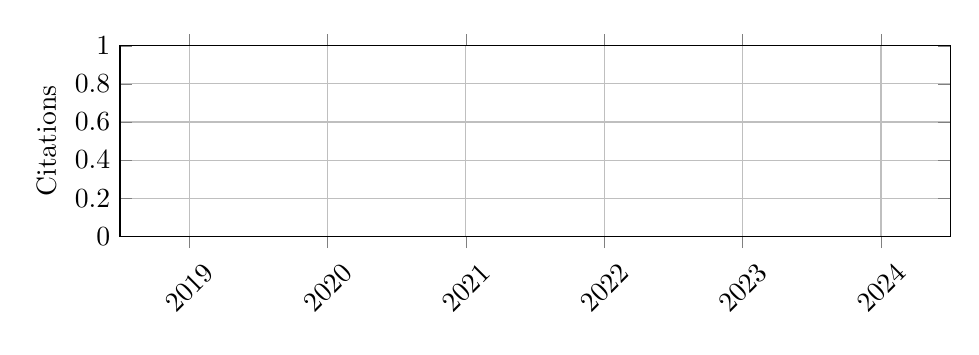
\begin{tikzpicture}
        \begin{axis}[
            width=\linewidth,% make the plot fill the subfigure width...
            height=4cm, % …but only 6 cm tall
            ybar,
            bar width=10pt,
            enlarge x limits=0.1,
            ylabel={\aiGoogleScholar Citations},
            ymin=0, ymax=220,
            ytick={ 0,55,110,165,220 },
            xtick=data,
            xticklabels={ 2018,2019,2020,2021,2022,2023,2024,2025 },
            % rotate the x‐tick labels:
            xticklabel style={rotate=45,anchor=near xticklabel},
            grid=major
          ]
          \                                                                  addplot[fill=gray] coordinates { (2018,41) (2019,67) (2020,151) (2021,171) (2022,207) (2023,168) (2024,184) (2025,57) };
        \end{axis}
      \end{tikzpicture}
    \end{subfigure}
  \end{figure}
%  \end{document}
\vspace{0.2 cm}   
    %\nocite{*}
    %\printbibliography
    %\printbibheading
\vspace{0.2 cm}    
\subsection{Journal Articles}
\csnumgdef{entrycount}{0}
\nocite{*}
\newrefcontext[labelprefix=J]
\printbibliography[env=counter,type=article,heading=none]
  \printbibliography[type=article,heading=none]
  
\subsection{Conference Proceedings}
\csnumgdef{entrycount}{0}
\nocite{*}
\newrefcontext[labelprefix=C]
\printbibliography[env=counter,type=inproceedings,heading=none]
\printbibliography[type=inproceedings,heading=none]


\subsection{Patents}
\csnumgdef{entrycount}{0}
\nocite{*}
\newrefcontext[labelprefix=P]
\printbibliography[env=counter,type=patent,heading=none]
\printbibliography[type=patent,heading=none]

\subsection{Preprint / Manuscript Under Preparation}
\csnumgdef{entrycount}{0}
\nocite{*}
\newrefcontext[labelprefix=X]
\printbibliography[env=counter,type=unpublished,heading=none]
\printbibliography[type=unpublished,heading=none]


\section{Membership / Fellowship of Learned Societies, Professional Institutions and Other Noteworthy Affiliations}
        \begin{onecolentry}
            \textbf{Senior Member, Institute of Electrical and Electronic Engineers (IEEE)}
            \begin{highlights}
                \item Secretary, IEEE Bangladesh Section (July 2021 - May 2022)
                \item Chair, IEEE Young Professionals Bangladesh	(Mar 2020 - Apr 2022)
                \item Chair, IEEE Graduates of the Last Decade	(Jan 2013 - Dec 2013)
                \item Vice -Chair, IEEE Graduates of the Last Decade	(Jan 2011 - Dec 2012)
                \item Student Activities Coordinator, IEEE Bangladesh Section	(Jan 2011 - Dec 2012)
                \item Chair, IEEE BUET Student Branch	(Jan 2008 - Aug 2009)
                \item Treasurer, IEEE BUET Student Branch	(Jan 2007 - Dec 2008)
            \end{highlights}
        \end{onecolentry}
        \begin{onecolentry}
            \textbf{Member, IEEE Photonics Society}
            \begin{highlights}
                \item Vice Chair, IEEE Photonics Society Bangladesh	(April 2022 – to date)
                \item Founding Chair, IEEE Photonics Society Bangladesh	(Mar 2021 – Apr 2022)
                \end{highlights}
            \end{onecolentry}
            \begin{onecolentry}
                \textbf{Member, The Optica}
                \begin{highlights}
                \item Founding President, Optica Bangladesh Section	May 2022 – to date
                \item Founding Moderator, BUET Optical and Photonics Society 	July 2022 – to date 
                \item Treasurer, OSA Purdue Chapter, USA	Jun 2016 – May 2017
            \end{highlights}
            \end{onecolentry}        
            \begin{onecolentry}
                \textbf{Member, National Young Academy of Bangladesh (NYAB)}, April 2021 – to date    \\     
                \textbf{Life Member, American Alumni Association of Bangladesh (AAAB)	}, April 2024 – to date    
                \\                    
                \textbf{Life Member, Association of BUET Alumni}, April 2021 – to date    \\     

        \end{onecolentry} 
        \begin{onecolentry}
            \textbf{Student Activities at Purdue University}, West Lafayette, IN, USA
            \begin{highlights}
                \item President, \textbf{Nanotechnology Student Advisory Council (NSAC)}	(Jun 2017 – May 2018)
                \item Vice-President, \textbf{Nanotechnology Student Advisory Council (NSAC)}	(Jun 2016 – May 2017)
                \item Treasurer, SPIE Purdue Chapter, USA (Jun 2015 – May 2016)
                \item President, Bangladesh Students Association (\textbf{Purdue BDSA}), USA  (Jul 2017 – Jun 2018)
                \item Treasurer, Bangladesh Students Association (\textbf{Purdue BDSA}), USA  (Jul 2015 – Jun 2017)
            \end{highlights}
        \end{onecolentry} 

        \vspace{0.2 cm}
    
\section{References}

Available upon request

    

\end{document}